\section{Results and Evaluation}
\label{header:results}

\paragraph{}This section presents the empirical evaluation of the implemented prototype against the four pillars established in Section~\ref{sect:meth4}: cryptographic correctness, performance, adversarial resilience, and end-user acceptance. The evaluation was conducted on the localhost build of the prototype, whose architecture is identical to the production deployment described in Section~\ref{sect:meth4_d}; the only material difference between the two environments is the addition of a TLS termination layer at the cloud edge, which does not affect the cryptographic protocol itself but does add fixed network round-trip overhead. All artifacts referenced in this section (i.e., raw test logs, statistical summaries, and the unaltered output of the benchmark scripts) are reproduced under the project's \texttt{logs/} directory and are referenced inline by listing.

\subsection{Functional and Cryptographic Validation}
\label{sect:results_func}

\paragraph{}Cryptographic correctness was assessed through a Vitest-based unit suite (under \texttt{server/tests/} as \texttt{functional.test.js}) that isolates the BLS12-381 primitives (i.e., hash-to-curve, partial signing, Lagrange-based aggregation, and bilinear-pairing verification) from the network and persistence layers. The suite executes thirty-five (35) tests across seven (7) categories and completed in 707~ms on the development machine. Results are summarised in Table~\ref{tab:functional}.

\begin{table}[H]
  \centering
  \caption{Functional test results: BLS12-381 primitives (35 / 35 passed).}
  \label{tab:functional}
  \begin{tabular}{|c|l|c|c|}
    \hline
    \# & Category & Tests & Result \\\hline
    1 & Hash function (\texttt{hashMessage}) & 5 & 5 / 5 \\\hline
    2 & Partial signature generation (\texttt{signMessage}) & 5 & 5 / 5 \\\hline
    3 & Threshold configuration & 6 & 6 / 6 \\\hline
    4 & All ten valid 3-of-5 combinations & 10 & 10 / 10 \\\hline
    5 & Insufficient signers (security) & 2 & 2 / 2 \\\hline
    6 & Tamper-resistance (payload attacks) & 6 & 6 / 6 \\\hline
    7 & Aggregation error handling & 1 & 1 / 1 \\\hline
    \multicolumn{2}{|r|}{\textbf{Total}} & \textbf{35} & \textbf{35 / 35} \\\hline
  \end{tabular}
\end{table}

\paragraph{}Particularly relevant to the threshold-correctness claim is Category~4: every one of the $\binom{5}{3} = 10$ possible 3-of-5 signer combinations was tested for end-to-end aggregation. Each subset successfully reconstructed the joint secret through Lagrange interpolation and produced an aggregate signature $F_{\text{sig}}$ that satisfied the bilinear pairing equation
\[
e(F_{\text{sig}},\, g) \;=\; e(H(M),\, PK).
\]

\paragraph{}Conversely, Category~5 confirmed the dual property: every 2-of-5 combination tested failed verification, since two evaluation points on the degree-2 polynomial $f(x) = \text{secret} + x + x^2$ uniquely determine a degree-1 line that does not pass through $f(0) = \text{secret}$. The Lagrange interpolation produces an arithmetically valid but cryptographically incorrect scalar, which the pairing equation rejects. This is the precise mathematical property that grounds the threshold-security claim of the protocol; a coalition of fewer than $t$ shareholders cannot forge a signature even with full knowledge of their own shares.

\paragraph{}Tamper-resistance (Category~6) addressed the integrity guarantee. Six payload attacks were attempted: amount tampering ($\textit{amount}: 2500 \to 1$), nonce replacement, timestamp zeroing, two forged-byte signatures (random hex and all-zero), and cross-transaction signature reuse. All six were rejected by the verifier, either by the curve membership check inside the underlying \texttt{@noble/curves} library (for malformed points such as the random and all-zero forgeries) or by the pairing equation itself (for valid points produced from a different message digest). In every case, the rejection was fail-closed: the verifier returned \texttt{false} without exposing any partial information about which check had failed, removing the oracle that an attacker would otherwise need to refine forged inputs.

\subsection{Performance Benchmarks}
\label{sect:results_perf}

\paragraph{}The latency benchmark, executed via \texttt{server/tests/latency-test.js}, measures the two performance-critical operations: (i) \textbf{QR generation}, defined as the time from the \texttt{request\_transaction} emission to receipt of \texttt{transaction\_initiated} with status \texttt{COMPLETED}; and (ii) \textbf{payment verification}, the time from the \texttt{verify\_payment} emission to receipt of \texttt{payment\_processed}. Each trial used a single low-value transaction (₱100--₱109, threshold $t = 1$) with a 300~ms inter-trial delay to avoid lock contention on the per-transaction mutex. Thirty (30) consecutive trials were collected.

\begin{table}[H]
  \centering
  \caption{Latency benchmark (\textit{n} = 30). Acceptance criterion: verification $< 200$~ms.}
  \label{tab:latency}
  \begin{tabular}{|l|c|c|c|}
    \hline
    Metric & QR Generation & Verification & Total End-to-End \\\hline
    $n$ & 30 & 30 & 30 \\\hline
    Min & 19~ms & 3~ms & 23~ms \\\hline
    Max & 32~ms & 8~ms & 36~ms \\\hline
    Mean & 24.73~ms & 4.83~ms & 29.57~ms \\\hline
    Std.\ dev. & 2.87~ms & 1.21~ms & 2.81~ms \\\hline
    Median (p50) & 24~ms & 5~ms & 29~ms \\\hline
    p90 & 29~ms & 7~ms & 34~ms \\\hline
    p95 & 31~ms & 7~ms & 34~ms \\\hline
    p99 & 32~ms & 8~ms & 36~ms \\\hline
  \end{tabular}
\end{table}

\paragraph{}\textbf{a.) Verification latency.} The principal acceptance criterion of Section~\ref{sect:meth4_c} --- has a sample mean of $4.83$~ms and a 99th-percentile worst case of $8$~ms across 30 trials. Every trial completed in well under $200$~ms; the 99th-percentile margin against the target is $200 / 8 = 25\times$. This margin is large enough that even on the production cloud deployment, where geographic routing on the free-tier hosting introduces an additional $50$--$150$~ms of round-trip overhead, the total verification time is expected to remain well within the criterion.

\paragraph{}\textbf{b.) QR generation.} This is the more expensive of the two operations because it bundles three cryptographic primitives, namely, BLS partial signing, Lagrange-based aggregation, and bilinear-pairing self-verification, with a sequence of MongoDB writes (\texttt{Transaction.create}, \texttt{Transaction.save}, \texttt{GroupBalance.findOneAndUpdate}, \texttt{AuditLog.save}). Even so, the mean of $24.73$~ms and the p99 of $32$~ms remain comfortably below the $100$~ms threshold conventionally taken as the upper bound of imperceptible response in interactive systems. Figure~\ref{fig:latency-dist} visualises the distribution of the verification path against the acceptance criterion, and Listing~\ref{lst:latency} reproduces the relevant excerpt of the benchmark output verbatim, for traceability.

\begin{figure}[H]
  \centering
  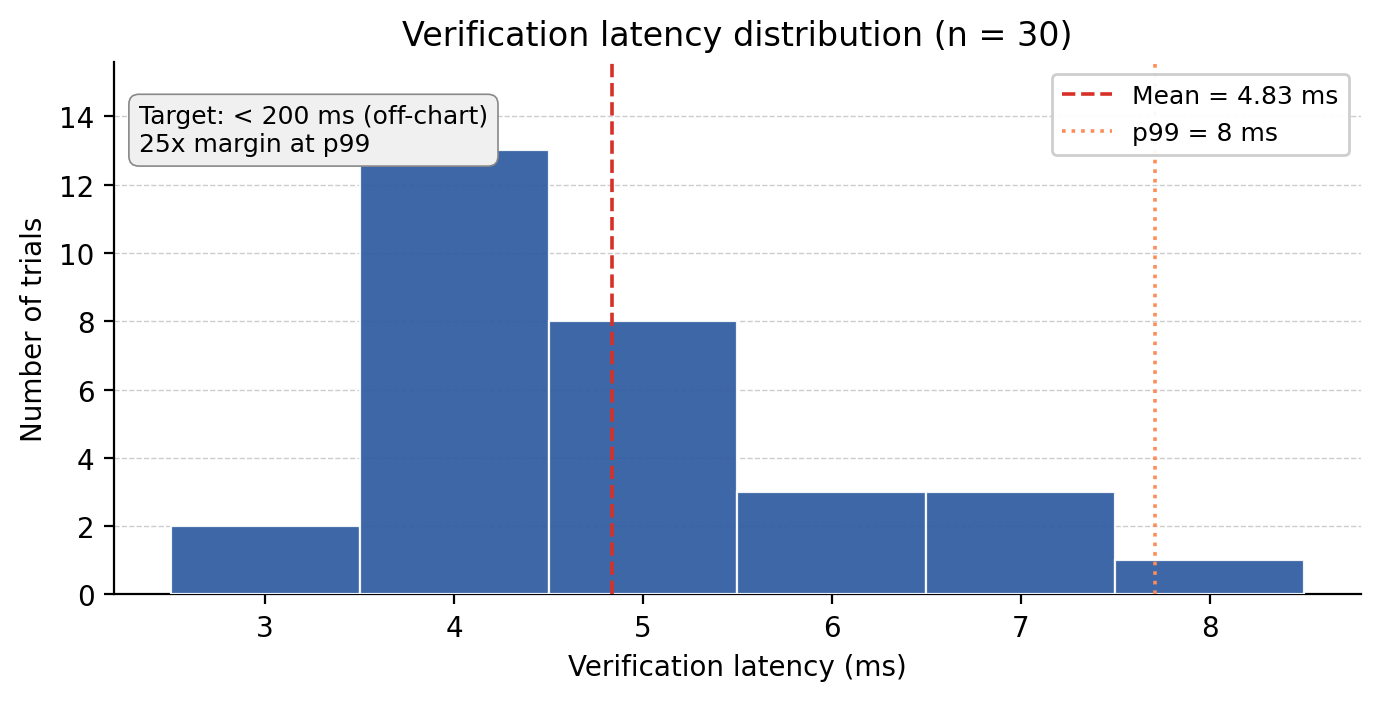
\includegraphics[width=0.85\textwidth]{images/fig_latency.png}
  \caption{Verification latency distribution over $n = 30$ trials. The acceptance criterion ($< 200$~ms) lies far off-chart; every observed sample is comfortably below it, with a $\sim 25\times$ margin at the 99th percentile.}
  \label{fig:latency-dist}
\end{figure}

\begin{lstlisting}[caption={Excerpt of the latency benchmark output (\texttt{npm run test:latency}, 30 trials, 2026-05-02).}, label={lst:latency}]
Verification Latency
Metric       Value
-------------------------
n            30
min          3 ms
max          8 ms
mean         4.83 ms
std dev      1.21 ms
p50          5 ms
p90          7 ms
p95          7 ms
p99          8 ms

Total End-to-End Latency
Metric       Value
-------------------------
mean         29.57 ms
p95          34 ms
p99          36 ms

TARGET CHECK: Verification latency < 200 ms
Passed: 30/30 trials (100.0%)
Result: PASS  (p95 = 7 ms)
\end{lstlisting}

\paragraph{}A complementary observation concerns the BLS aggregation step itself. Because BLS signatures aggregate into a single compact group element regardless of the number of signers, the \textit{post}-aggregation payload size is invariant in $t$; only the pre-aggregation message complexity grows linearly with $t$, and that growth is absorbed entirely on the server. This is a structural advantage over multi-signature schemes that concatenate independent signatures into the QR payload (e.g., stacked RSA), where increasing $t$ inflates QR data density and consequently scan latency, as further discussed in Section~\ref{sect:disc_qr}.

\subsection{Adversarial / MITM Validation}
\label{sect:results_mitm}

\paragraph{}Resilience against the threat model of Section~\ref{sect:meth4_b} was evaluated through the script under \texttt{ server/tests/} as \texttt{mitm-test.js}, which exercises thirteen (13) distinct attack scenarios partitioned into an offline cryptographic group (A1--A7) and an online protocol group (B1--B6). All thirteen scenarios resolved as expected; in each adversarial case the attack was blocked, and in the two positive controls (A7 and B4) the legitimate request was correctly accepted. Results are summarised in Table~\ref{tab:mitm}.

\begin{table}[H]
  \centering
  \caption{MITM attack scenarios: 13 / 13 resolved as expected.}
  \label{tab:mitm}
  \begin{tabular}{|c|l|c|}
    \hline
    \# & Scenario & Outcome \\\hline
    A1 & BLS forgery: random bytes as signature & Blocked \\\hline
    A2 & BLS forgery: all-zero signature bytes & Blocked \\\hline
    A3 & Amount tampering on a valid signature & Blocked \\\hline
    A4 & Nonce replacement on a valid signature & Blocked \\\hline
    A5 & Cross-transaction signature reuse & Blocked \\\hline
    A6 & 2-of-5 threshold attack & Blocked \\\hline
    A7 & Positive control (legitimate 3-of-5 sig) & Accepted \\\hline
    B1 & \texttt{verify\_payment} with nonexistent nonce & Blocked \\\hline
    B2 & Amount inflation (₱999{,}999 vs.\ stored ₱100) & Blocked \\\hline
    B3 & Amount deflation (₱1 vs.\ stored ₱500) & Blocked \\\hline
    B4 & Positive control (legitimate verify) & Accepted \\\hline
    B5 & Replay of a \texttt{PAID} transaction & Blocked \\\hline
    B6 & Premature verify (\texttt{PENDING} transaction) & Blocked \\\hline
  \end{tabular}
\end{table}

\paragraph{}\textbf{Offline cryptographic attacks (A1--A7)} target the pairing-verification logic directly without going through the WebSocket transport. A1 and A2 exercise the elliptic-curve membership check inside \texttt{@noble/curves}: a candidate pair $(x, y)$ that does not satisfy the BLS12-381 curve equation is rejected before the pairing computation begins, surfaced internally as \texttt{Error: bad point coordinate x} (random bytes) or \texttt{Error: bad point coordinate y} (all-zero bytes). A3--A5 hold the signature constant while perturbing the message digest $H(M)$ via amount tampering, nonce replacement, or cross-transaction signature reuse; in each case the pairing equation breaks because the signature was bound to a different digest. A6 directly tests the threshold property by aggregating only two of the five shares and presenting the result as if it were a complete signature; the Lagrange interpolation produces a scalar that does not equal the joint secret, and the pairing fails. A7 confirms the positive control: a legitimate aggregate of three shares verifies.

\paragraph{}\textbf{Online protocol attacks (B1--B6)} target the verifier through the same Socket.io interface a real client would use. B1 submits a freshly generated UUID as a transaction nonce; the verifier responds \texttt{``Transaction not found or has expired from records.''} since no matching ledger entry exists, demonstrating that nonce uniqueness alone is sufficient to defeat the simplest replay variants. B2 and B3 are the most economically meaningful attacks in the suite: an adversary who has compromised the WebSocket transport may attempt to inflate or deflate the deducted amount by submitting a forged \texttt{amount} field together with an otherwise valid (replayed) nonce. The current implementation deducts only the amount stored server-side at the time of transaction creation; the client-supplied value is logged but ignored. Test~B2 confirmed that a ₱999{,}999 inflation attempt against a ₱100 transaction resulted in exactly ₱100 being deducted; B3 confirmed the symmetric deflation case (₱1 submitted against a ₱500 transaction $\to$ ₱500 deducted). B5 verifies that a previously paid transaction (status \texttt{PAID}) cannot be re-verified; B6 verifies that a transaction whose threshold has not yet been met (status \texttt{PENDING}) cannot be paid out prematurely.

\paragraph{}\textit{A note on disclosure.} The amount-tampering vulnerability that motivated tests B2 and B3 was discovered during this study and patched in \texttt{server/controllers/socketHandler.js} prior to the performance benchmarking reported in Section~\ref{sect:results_perf}. The pre-fix handler used \texttt{data.amount} (the client-supplied value) as the operand of the balance deduction, exposing the system to an attacker who had broken the transport layer (e.g., via a rogue certificate authority or a downgrade attack on a non-TLS instance). The patched handler reads the authoritative amount from the persisted \texttt{Transaction} document, removing the client controllability of that field. The B2 and B3 tests were authored specifically to provide regression coverage for this fix.

\paragraph{}On the production deployment (\texttt{https://thesis-qr.onrender.com}), all Socket.io traffic uses WebSocket Secure (\texttt{wss://}) over TLS 1.3. A network-level adversary intercepting TCP packets observes only ciphertext, so the offline cryptographic attacks A1--A7 and the protocol attacks B1--B6 effectively assume an attacker who has already broken TLS, which is a strictly stronger threat model than a passive eavesdropper. The fact that all thirteen scenarios are still defeated under that stronger assumption is, in the view of the authors, the most consequential security claim of the present study.

\subsection{User Acceptance Testing (UAT)}
\label{sect:results_uat}

\paragraph{}The UAT followed the protocol set out in Section~\ref{sect:meth4_c}. A total of ten (10) participants were recruited and split into two groups of five (5) each, corresponding to a between-subjects A/B treatment of the QR code's data density. Group~A interacted with a higher-density (``Big QR'') variant of the dynamic code, in which the entire authorization payload (i.e., joint public key $PK$, generator $g$, aggregate signature $F_{\text{sig}}$, and transaction message $M$) was embedded directly in the QR matrix, yielding a self-contained, in-band cryptographic proof. Group~B used a smaller (``Small QR'') variant in which the same payload was identified by a short reference token, with the cryptographic content fetched out of band by the verifier upon scan. The two variants were therefore placed on opposite ends of a security--scannability axis: Big QR is fully self-contained and resistant to lookup-channel compromise but requires the camera to discriminate a denser module grid; Small QR is sparser and faster to scan but places trust in a separate retrieval path.

\paragraph{}Each participant was assigned a phone role, namely, Shopper (initiator), Approver, or Cashier (verifier), and walked through the ten test scenarios listed in the UAT instrument. Every scenario produced the expected outcome in both groups (\textbf{10 / 10 PASS} for each of A and B), including the race-condition case (Scenario~4: three approvers tap simultaneously on a ₱2{,}000 request; the system accepts the first two valid approvals and ignores the third), the double-scan-prevention case (Scenario~5), and the timeout / QR-expiry case (Scenario~9, in which the Shopper's screen showed ``request expired'' after the two-minute QR TTL had elapsed). Two scenarios are particularly worth flagging for the discussion that follows:

\begin{itemize}
  \item \textbf{Scenario~6 (Expired QR Code).} Although the test passed, an observer note flagged that the participant ``just need[ed] to open the QR \textit{agad}'' --- i.e., that the perceived window between QR generation and scan was tighter than the formal two-minute TTL would suggest. This anticipates the friction discussion in Section~\ref{sect:disc_qr}.
  \item \textbf{Scenario~7 (Fake / External QR).} The cashier app correctly rejected an unrelated GCash QR sticker, demonstrating that the verifier's payload-schema check (presence of $\{PK,\, g,\, F_{\text{sig}},\, M\}$) provides a usable second line of defence even before the pairing equation is evaluated. This is operationally important because it allows the verifier to discriminate ``not one of ours'' QRs without expending the cost of a pairing computation on every scan.
\end{itemize}

\subsubsection{System Usability Scale (SUS)}
\label{sect:results_uat_sus}

\paragraph{}A six-item adaptation of the System Usability Scale~\cite{brooke1996sus} was administered to all ten participants. Five items were positively keyed: frequency of intended use, ease of use, integration of functions, learnability, and perceived security. Contrarily, one item was negatively keyed (need for technical support to operate the system). Each was rated on a 5-point Likert scale.

\paragraph{}All five positively keyed items received unanimous ratings in the 4--5 range across both groups, indicating strong agreement with the system's usability claims. The negatively keyed item, ``\textit{I think that I would need the support of a technical person to use this system}'', received a unanimous rating of 1 (Strongly Disagree) from every participant in both groups, indicating that no participant perceived a need for technical assistance. Following the standard SUS scoring convention~\cite{brooke1996sus, bangor2008sus}, in which each positive item contributes ($\textit{rating} - 1$) and each negative item contributes ($5 - \textit{rating}$), the per-item contribution for every item in this study lies in the closed interval $[3, 4]$ out of a maximum of $4$. The aggregate normalised score, computed as
\[
\textit{SUS}_{6} \;=\; \frac{\sum_{i=1}^{6} c_i}{6 \times 4} \times 100,
\]
where $c_i$ denotes the per-item contribution, falls within the band $[87.5,\, 100]$. Although this six-item adaptation departs from the canonical 10-item instrument and the resulting scale is not strictly interchangeable with normative SUS benchmarks, the result situates the prototype well above the conventional ``excellent'' threshold of 80~\cite{bangor2008sus}.

\subsubsection{QR Recognition: A/B Findings}
\label{sect:results_uat_qr}

\paragraph{}Survey item~4.2 (``\textit{Did the Cashier's scanner recognise the dynamic QR code on the first attempt?}'') is the principal source of the A/B observation. The aggregated responses are reported in Table~\ref{tab:qr-recognition} and visualised in Figure~\ref{fig:qr-recognition}.

\begin{table}[H]
  \centering
  \caption{QR recognition survey results (Item 4.2) by group, $n = 5$ per group.}
  \label{tab:qr-recognition}
  \begin{tabular}{|l|c|c|}
    \hline
    Response & Group~A (Big QR) & Group~B (Small QR) \\\hline
    Yes, immediately & 2 / 5 (40\%) & 3 / 5 (60\%) \\\hline
    Took 2--3 seconds to focus & 3 / 5 (60\%) & 2 / 5 (40\%) \\\hline
    Failed / required retry & 0 / 5 & 0 / 5 \\\hline
  \end{tabular}
\end{table}
\begin{figure}[ht]
    \centering
    \begin{tikzpicture}
        \begin{axis}[
            ybar=2pt, % slight spacing between the grouped bars
            bar width=22pt, % width of the bars
            width=12cm,
            height=7.5cm,
            % Title formatting - Single line and explicitly centered
            title={\Large UAT Item 4.2 --- Did the cashier's scanner recognize the QR\\[1ex] on the first attempt?},
            title style={align=center, font=\sffamily, yshift=2ex},
            % Y-axis configuration
            ymin=0, 
            ymax=5,
            ytick={0,1,2,3,4,5},
            ymajorgrids=true,
            grid style={solid, gray!30},
            % X-axis configuration
            xmin=0.5, 
            xmax=3.5,
            xtick={1,2,3},
            xticklabels={{Yes, Immediately}, {Took 2-3 s to focus}, {Failed / retry}},
            % Ensure x-axis tick text is centered if it spans multiple lines
            tick label style={font=\sffamily\small, color=darkgray, align=center},
            % Hide default axis lines and ticks to match the clean look
            axis line style={draw=none},
            tick style={draw=none},
            % Manually draw the bottom x-axis line
            before end axis/.code={
                \draw [gray!40] ({rel axis cs:0,0}) -- ({rel axis cs:1,0});
            },
            % Legend configuration
            legend style={
                at={(0.5,-0.15)},
                anchor=north,
                legend columns=-1, % horizontal legend
                draw=none, % remove legend border
                font=\sffamily\small\color{darkgray},
                /tikz/every even column/.append style={column sep=0.5cm} % spacing
            }
        ]
        
        % Data for Group A (Big QR)
        \addplot[fill=groupAblue, draw=none] coordinates {
            (1,2) 
            (2,3) 
            (3,0)
        };
        
        % Data for Group B (Small QR)
        \addplot[fill=groupBorange, draw=none] coordinates {
            (1,3) 
            (2,2) 
            (3,0)
        };
        
        % Proper curly braces to prevent comma separation issues
        \legend{{Group A (Big QR, n=5)}, {Group B (Small QR, n=5)}}
        \end{axis}
    \end{tikzpicture}
    
    % --- Added Caption and Label here ---
    \caption{QR recognition responses by group (UAT Item 4.2). The 60\%~/~40\% split on the ``2--3 seconds to focus'' bin is the principal source of the A/B finding discussed in Section~\ref{sect:disc_qr}.}
    \label{fig:qr-recognition}
\end{figure}


\paragraph{}A 2--3 second focus delay was reported by a majority of the Group~A participants but only a minority of participants in Group B. This is consistent with the well-documented relationship between QR module density and camera autofocus latency: as the density of black/white modules per linear inch rises (a function of QR version and physical display size), the camera must focus more precisely to discriminate adjacent modules, and the autofocus algorithm typically requires more frames to settle~\cite{corpuz2025}. The Big QR variant in this study used QR versions that pack the entire $\sim 440$-byte cryptographic payload (the joint public key $PK$, the aggregate signature $F_{\text{sig}}$, the curve generator $g$, and the message $M$) directly into the matrix --- realised here as a version-14 QR with $77 \times 77$ modules; the Small QR variant used a much sparser version-2 QR ($25 \times 25$ modules) carrying only a short reference token, and its payload size is essentially independent of $t$. The observation is symmetric across participants and consistent with the protocol's structural choice of in-band versus out-of-band cryptographic content. No participant in either group reported a hard scan failure, which is the relevant binary acceptance criterion for the prototype; the 2--3 second penalty is a usability signal rather than a correctness one.

\subsubsection{Perceived Security and Open-Ended Feedback}
\label{sect:results_uat_open}

\paragraph{}On Section~5 of the survey (``Multi-Party Approval''), all ten participants selected either ``Yes, significantly safer'' or ``Somewhat safer'' when asked whether the requirement for multi-party approval increased their perception of the system's safety against unauthorised spending. No participant selected the ``No difference'' or ``No, it felt less secure'' options. 

\begin{figure}[ht]
    \centering
    \begin{tikzpicture}
        \begin{axis}[
            ybar=2pt, % slight spacing between the grouped bars
            bar width=22pt, % width of the bars
            width=12cm,
            height=7.5cm,
            % Title formatting - Single line and explicitly centered
            title={\Large UAT Item 5.1 --- Did knowing that multiple people had to approve \\[0.5ex] the transaction make you feel safer against unauthorized spending?},
            title style={align=center, font=\sffamily, yshift=2ex},
            % Y-axis configuration
            ymin=0, 
            ymax=5,
            ytick={0,1,2,3,4,5},
            ymajorgrids=true,
            grid style={solid, gray!30},
            % X-axis configuration
            xmin=0.5, 
            xmax=4.5,
            xtick={1,2,3,4},
            xticklabels={{Yes, significantly safer}, {Somewhat safer}, {No difference}, {No, it felt less secure}},
            % Ensure x-axis tick text is centered if it spans multiple lines
            tick label style={font=\sffamily\small, color=darkgray, align=center, text width=2.5cm},
            % Hide default axis lines and ticks to match the clean look
            axis line style={draw=none},
            tick style={draw=none},
            % Manually draw the bottom x-axis line
            before end axis/.code={
                \draw [gray!40] ({rel axis cs:0,0}) -- ({rel axis cs:1,0});
            },
            % Legend configuration
            legend style={
                at={(0.5,-0.25)},
                anchor=north,
                legend columns=-1, % horizontal legend
                draw=none, % remove legend border
                font=\sffamily\small\color{darkgray},
                /tikz/every even column/.append style={column sep=0.5cm} % spacing
            }
        ]
        
        % Data for Group A (Big QR)
        \addplot[fill=groupAblue, draw=none] coordinates {
            (1,4) 
            (2,1) 
            (3,0)
            (4,0)
        };
        
        % Data for Group B (Small QR)
        \addplot[fill=groupBorange, draw=none] coordinates {
            (1,1) 
            (2,4) 
            (3,0)
            (4,0)
        };
        
        % Proper curly braces to prevent comma separation issues
        \legend{{Group A (Big QR, n=5)}, {Group B (Small QR, n=5)}}
        \end{axis}
    \end{tikzpicture}
    
    % --- Added Caption and Label here ---
    \caption{Survey results for the perceived safety of the QR system}
    \label{fig:qr-recognition}
\end{figure}


This finding is consistent with the literature on mental models of multi-party authorisation~\cite{komlo2021}, which reports that visible enforcement of an approval quorum tends to dominate perceived security over the underlying cryptographic mechanism, regardless of whether participants understand the latter.

\paragraph{}Two recurring suggestions emerged from the open-ended feedback (Section~7.1 of the survey instrument):

\begin{enumerate}
  \item \textbf{A Deposit / fund-replenishment feature.} Several participants observed that the prototype currently models only the spending side of a joint account: members can debit the shared balance subject to threshold approval, but there is no symmetric flow for crediting it. Participants asked whether large \textit{deposits} should also require multi-party acknowledgement (for instance, to prevent a single member from quietly retitling external funds into the joint account) or whether deposits should be permissive by default. This is treated as Recommendation~\ref{sect:rec_deposit}.
  \item \textbf{Stricter credential confirmation at the point of approval.} Several participants observed that, in the current prototype, possession of an unlocked phone is functionally equivalent to consent to sign, i.e., a tap on the ``Approve'' button produces a partial signature without any further authentication step. Suggestions included a per-approval password prompt, a biometric confirmation (fingerprint or Face~ID), or a short PIN. This is treated as Recommendation~\ref{sect:rec_mfa}.
\end{enumerate}

\paragraph{}On the overall recommendation question (Section~7.2), all ten participants stated they would consider using or recommending the system for a real joint account, with several volunteering the multi-party approval mechanism as the central reason. No participant offered a strictly negative recommendation.

\subsection{Consolidated Evaluation}
\label{sect:results_summary}

\paragraph{}Table~\ref{tab:results-summary} consolidates the headline outcomes against the acceptance criteria stated in Section~\ref{sect:meth4}. Every quantitative criterion was satisfied with substantial margin, and every qualitative criterion (UAT scenario coverage, SUS, perceived security) returned a positive verdict. The principal qualitative caveat to the result is the QR scan-latency observation in the Big QR condition, which motivates the recommendations of Section~\ref{header:recs}.

\begin{table}[H]
  \centering
  \caption{Consolidated evaluation against acceptance criteria.}
  \label{tab:results-summary}
  \begin{tabular}{|l|l|l|c|}
    \hline
    Stream & Criterion & Measured & Status \\\hline
    Functional & Unit-test pass rate & 35 / 35 (100\%) & Pass \\\hline
    Functional & All 3-of-5 combinations verify & 10 / 10 & Pass \\\hline
    Functional & Tampered payloads rejected & 6 / 6 & Pass \\\hline
    Performance & Verification mean & 4.83~ms ($< 200$~ms) & Pass \\\hline
    Performance & Verification p99 & 8~ms ($< 200$~ms) & Pass \\\hline
    Performance & Trials under 200~ms & 30 / 30 (100\%) & Pass \\\hline
    Adversarial & Cryptographic attacks blocked & 7 / 7 & Pass \\\hline
    Adversarial & Protocol attacks blocked & 6 / 6 (incl.\ 2 positive controls) & Pass \\\hline
    UAT & Scenario coverage (each group) & 10 / 10 & Pass \\\hline
    UAT & Modified six-item SUS aggregate & 87.5--100 band & Pass \\\hline
    UAT & Perceived multi-party safety & 10 / 10 positive & Pass \\\hline
  \end{tabular}
\end{table}
